\documentclass[a4paper,12pt]{jsreport}
\usepackage{bm}
\usepackage[dvipdfmx]{graphicx}
\usepackage{here}
\usepackage{ascmac}
\usepackage{comment}
\usepackage{multirow}
\usepackage{graphics}
\usepackage{graphicx}
\usepackage{scalefnt}
\usepackage{mathtools}
\setcounter{secnumdepth}{4}


\title{タンパク質のアミノ酸配列間距離の評価のための\\
最適なベクトルの割り当て}
\author{土山啓汰\\
弘前大学理工学部電子情報工学科}

% \date{2020年吉日}

\begin{document}
\maketitle
\tableofcontents


\chapter{イントロダクション}

\section{研究の背景と目的}
本研究ではタンパク質のアミノ酸配列を扱う。アミノ酸はタンパク質の構成要素である。20種類の異なるアミノ酸がタンパク質の合成に用いられる。各タンパク質の形状や他の特性はそこに含まれるアミノ酸の配列の仕方によって決定し、アミノ酸配列が似ているほど機能や性質が類似している可能性が高いと言える。 \\
タンパク質のアミノ酸配列間の類似性を評価する方法として、一般的にアライメントが用いられている。しかし、配列長が$N$と$N$の場合は動的計画法により$O(N^2)$の時間計算量となり、肥大な計算時間が必要となる。そのため、本研究室ではアライメントに依らないタンパク質アミノ酸配列比較の手法として、アミノ酸に何らかの2次元ベクトルを割り当てグラフィカル表現を行うことが提案されてきた。これにより、グラフが似ていれば類似性が高いといったような直観的な評価が可能となる。また、同時に定量的な評価も行う。\\
 本研究では、この手法の精度を高めるために、アミノ酸のベクトルの割り当て方に注目し、遺伝子解析同等の系統樹を早く作成することを目的としている。


\chapter{方法}

\section{ベクトルの割り当て}

タンパク質のアミノ酸配列を3次元座標群化するためにアミノ酸20種にベクトルを割り当てる。本研究では、疎水性度、コドン表、等電点を元に割り当てることにした。

\subsection{疎水性度}
アミノ酸を疎水性度をもとにして配置する。また、疎水性度はModified Kyte-Doolittle hydrophobicity scale (Juretic et al., 1998)を参考にする。


\begin{table}[H]
\centering
\caption{疎水性度表}
\scalebox{1}[1]{
\begin{tabular}{|cc|cc|} \hline
アミノ酸 & 疎水性度 & アミノ酸 & 疎水性度 \\ \hline
R & -5.10 &G & -0.64 \\[-2mm]
K & -4.11 &S & -0.50 \\[-2mm]
Q & -3.68 &W & -0.46 \\[-2mm]
D & -3.60 &A & 1.10 \\[-2mm]
N & -3.50 &M & 1.90 \\[-2mm]
H & -3.20 &C & 2.50 \\[-2mm]
E & -3.20 &F & 2.80 \\[-2mm]
P & -1.90 &L & 3.80 \\[-2mm]
Y & -1.30 &V & 4.20 \\[-2mm]
T & -0.70 &I & 4.50 \\ \hline
\end{tabular}
}
\end{table}


\subsubsection{アミノ酸を疎水性度の値が小さい順に、内側、外側に10種類ずつ二重円で配置}
開始位置はArg(R)で、時計回りとする。


\begin{figure}[H]
\centering
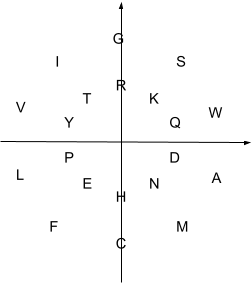
\includegraphics[width=50mm]{pic01.png}
\caption{XY平面上の配置}
\end{figure}


\begin{table}[H]
\centering
\caption{アミノ酸の座標値}
\scalebox{1}[1]{
\begin{tabular}{|cccc|cccc|} \hline
アミノ酸(内側) & x & y & z & アミノ酸(外側) & x & y & z \\ \hline
R & 0.000 & 1.257 & 1.257 & G & 0.000 & 2.300 & 1.150\\[-2mm]
K & 0.727 & 1.000 & 1.236 & S & 1.385 & 1.906 & 1.178 \\[-2mm]
Q & 1.336 & 0.434 & 1.405 & W & 3.726 & 1.211 & 1.959 \\[-2mm]
D & 1.201 & -0.390 & 1.263 & A & 2.060 & -0.669 & 1.083 \\[-2mm]
N & 0.818 & -1.125 & 1.391 & M & 1.902 & -2.616 & 1.617 \\[-2mm]
H & 0.000 & -1.643 & 1.643 & C & 0.000 & -3.718 & 1.859 \\[-2mm]
E & -0.689 & -0.948 & 1.172 & F & -1.662 & -2.286 & 1.413 \\[-2mm]
P & -1.259 & -0.409 & 1.324 & L & -1.930 & -0.627 & 1.015 \\[-2mm]
Y & -1.460 & 0.474 & 1.535 & V & -2.212 & 0.719 & 1.163 \\[-2mm]
T & -0.747 & 1.028 & 1.271 & I & -1.444 & 1.987 & 1.228 \\ \hline
\end{tabular}
}
\end{table}




\subsubsection{アミノ酸を疎水性度の値が小さい順に、疎水性度の値がプラスとマイナスで分けて二重円に配値}
開始位置はArg(R)で、時計回りとする。

\begin{figure}[H]
\centering
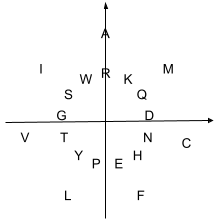
\includegraphics[width=53mm]{pic02.png}
\caption{XY平面上の配置}
\end{figure}

\begin{table}[H]
\centering
\caption{アミノ酸の座標値}
\scalebox{1}[1]{
\begin{tabular}{|cccc|cccc|} \hline
アミノ酸(内側) & x & y & z & アミノ酸(外側) & x & y & z \\ \hline
R & 0.000 & 1.257 & 1.257 & A & 0.000 & 2.166 & 1.083 \\[-2mm]
K & 0.575 & 1.094 & 1.236 & M & 1.301 & -0.494 & 1.617 \\[-2mm]
Q & 1.156 & 0.798 & 1.405 & C & 3.625 & -0.827 & 1.859 \\[-2mm]
D & 1.254 & 0.153 & 1.263 & F & 1.226 & -2.546 & 1.413 \\[-2mm]
N & -0.316 & -1.286 & 1.391 & L & 2.529 & 2.016 & 1.617 \\[-2mm]
H & 1.089 & -1.231 & 1.643 & V & -2.268 & -0.518 & 1.163 \\[-2mm]
E & 0.280 & -1.138 & 1.172 & I & -1.921 & 1.531 & 1.228 \\[-2mm]
P & 1.156 & 0.798 & 1.324 &&&& \\[-2mm]
Y & -1.018 & -1.150 & 1.535 &&&& \\[-2mm]
T & -1.188 & -0.451 & 1.271 &&&& \\[-2mm]
G & -1.142 & 0.139 & 1.150 &&&& \\[-2mm]
S & -0.969 & 0.669 & 1.178 &&&& \\[-2mm]
W & -0.915 & 1.734 & 1.959 &&&& \\ \hline
\end{tabular}
}
\end{table}

\subsubsection{アミノ酸を疎水性度の値が小さい順に、疎水性度の値がプラスとマイナスで分けて左右に配値}
開始位置はそれぞれArg(R)、Ala(A)とする。

\begin{figure}[H]
\centering
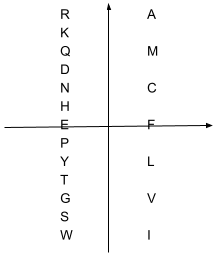
\includegraphics[width=53mm]{pic03.png}
\caption{XY平面上の配置}
\end{figure}

\begin{table}[H]
\centering
\caption{アミノ酸の座標値}
\scalebox{1}[1]{
\begin{tabular}{|cccc|cccc|} \hline
アミノ酸(内側) & x & y & z & アミノ酸(外側) & x & y & z \\ \hline
R & -1.257 & 7.542 & 1.257 & A & 1.083 & 6.498 & 1.083 \\[-2mm]
K & -1.236 & 6.180 & 1.236 & M & 1.617 & 6.468 & 1.617 \\[-2mm]
Q & -1.405 & 5.620 & 1.405 & C & 1.859 & 3.718 & 1.859 \\[-2mm]
D & -1.263 & 3.789 & 1.263 & F & 1.413 & 0.000 & 1.413 \\[-2mm]
N & -1.391 & 2.782 & 1.391 & L & 1.015 & -2.030 & 1.617 \\[-2mm]
H & -1.643 & 1.643 & 1.643 & V & 1.163 & -4.652 & 1.163 \\[-2mm]
E & -1.172 & 0.000 & 1.172 & I & 1.228 & -7.368 & 1.228 \\[-2mm]
P & -1.324 & -1.324 & 1.324 &&&& \\[-2mm]
Y & -1.535 & -3.070 & 1.535 &&&& \\[-2mm]
T & -1.271 & -3.813 & 1.271 &&&& \\[-2mm]
G & -1.150 & -4.600 & 1.150 &&&& \\[-2mm]
S & -1.178 & -5.890 & 1.178 &&&& \\[-2mm]
W & -1.959 & -11.754 & 1.959 &&&& \\ \hline
\end{tabular}
}
\end{table}



\subsection{コドン表}
アミノ酸をコドン表をもとにして配置する。表は3文字の大文字で書かれた塩基に、それぞれ対応するアミノ酸が書かれている(TERは終止コドン)。また、ロイシン(Leu)、アルギニン(Arg)、セリン(Ser)はコドン表に複数存在している。ロイシン、アルギニンは近い位置にあるため平均をとった位置とし、セリンは親水性であるため右下に配置した。

\begin{table}[H]
\centering
\caption{コドン表}
\scalebox{1}[1]{
\begin{tabular}{|lc|lc|lc|lc|} \hline
TTT & Phe & TCT & Ser & TAT & Tyr & TGT & Cys \\[-2mm] 
TTC & Phe & TCC & Ser & TAC & Tyr & TGC & Cys \\[-2mm]
TTA & Leu & TCA & Ser & TAA & TER & TGA & TER \\[-2mm]
TTG & Leu & TCG & Ser & TAG & TER & TGG & Trp \\ \hline
CTT & Leu & CCT & Pro & CAT & His & CGT & Arg \\[-2mm]
CTC & Leu & CCC & Pro & CAC & His & CGC & Arg \\[-2mm]
CTA & Leu & CCA & Pro & CAA & Gln & CGA & Arg \\[-2mm]
CTG & Leu & CCG & Pro & CAG & Gln & CGG & Arg \\ \hline
ATT & Ile & ACT & Thr & AAT & Asn & AGT & Ser \\[-2mm]
ATC & Ile & ACC & Thr & AAC & Asn & AGC & Ser \\[-2mm]
ATA & Ile & ACA & Thr & AAA & Lys & AGA & Arg \\[-2mm]
ATG & Met & ACG & Thr & AAG & Lys & AGG & Arg \\ \hline
GTT & Val & GCT & Ala & GAT & Asp & GGT & Gly \\[-2mm]
GTC & Val & GCC & Ala & GAC & Asp & GGC & Gly \\[-2mm]
GTA & Val & GCA & Ala & GAA & Glu & GGA & Gly \\[-2mm]
GTG & Val & GCG & Ala & GAG & Glu & GGG & Gly \\ \hline
\end{tabular}
}
\end{table}

\begin{figure}[H]
\centering
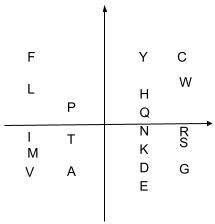
\includegraphics[width=53mm]{pic04.png}
\caption{XY平面上の配置}
\end{figure}


\begin{table}[H]
\centering
\caption{アミノ酸の座標値}
\scalebox{1}[1]{
\begin{tabular}{|cccc|cccc|} \hline
アミノ酸(内側) & x & y & z & アミノ酸(外側) & x & y & z \\ \hline
A & -4.332 & -6.498 & 1.083 & M & -12.936 & -5.659 & 1.617 \\[-2mm]
C & 14.872 & 13.013 & 1.859 & N & 5.564 & -1.391 & 1.391 \\[-2mm]
D & 5.052 & -6.315 & 1.263 & P & -5.296 & 2.648 & 1.324 \\[-2mm]
E & 4.688 & -8.204 & 1.172 & Q & 5.620 & 1.405 & 1.405 \\[-2mm]
F & -11.304 & 9.891 & 1.413 & R & 10.056 & -0.629 & 1.257 \\[-2mm]
G & 9.200 & -6.900 & 1.150 & S & 9.424 & -1.178 & 1.178 \\[-2mm]
H & 6.572 & 4.929 & 1.643 & T & -5.084 & -2.542 & 1.271 \\[-2mm]
I & -9.824 & -1.842 & 1.228 & V & -9.304 & -6.978 & 1.163 \\[-2mm]
K & 4.944 & -3.708 & 1.236 & W & 15.672 & 8.816 & 1.959 \\[-2mm]
L & -8.120 & 3.552 & 1.015 & Y & 6.140 & 10.745 & 1.535 \\ \hline
\end{tabular}
}
\end{table}


\subsection{等電点}
アミノ酸を等電点をもとにして配置する。等電点はIsoelectric point (Zimmerman et al., 1968)を参考にする。アミノ酸の配置は、等電点の値が小さい順に、内側、外側に10種類ずつ二重円で配置した。開始位置はArg(D)で、時計回りとする。

\begin{table}[H]
\centering
\caption{等電点}
\scalebox{1}[1]{
\begin{tabular}{|cc|cc|} \hline
アミノ酸 & 等電点 & アミノ酸 & 等電点 \\ \hline
D & 2.77 & W & 5.89 \\[-2mm]
E & 3.22 & V & 5.96 \\[-2mm]
C & 5.05 & G & 5.97 \\[-2mm]
N & 5.41 & L & 5.98 \\[-2mm]
F & 5.48 & A & 6.00 \\[-2mm]
Q & 5.65 & I & 6.02 \\[-2mm]
T & 5.66 & P & 6.30 \\[-2mm]
Y & 5.66 & H & 7.59 \\[-2mm]
S & 5.68 & K & 9.74 \\[-2mm]
M & 5.74 & R & 10.76 \\ \hline
\end{tabular}
}
\end{table}

\begin{figure}[H]
\centering
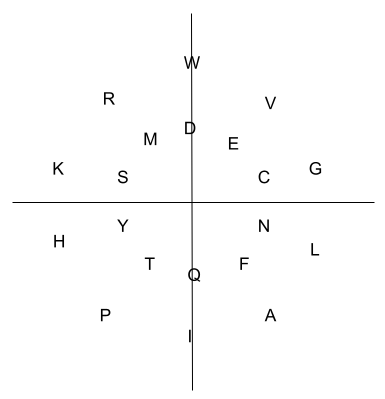
\includegraphics[width=53mm]{pic04x.png}
\caption{XY平面上の配置}
\end{figure}

\newpage
\section{三次元座標群の作成}
アミノ酸に割り当てたベクトルを元に三次元座標群を作成する。例として配列ACDEFに対する座標群を表2.8に示す。

\begin{table}[h]
\centering
\caption{3次元座標群の例}
\scalebox{1}[1]{
\begin{tabular}{c|lll}\hline
&X&Y&Z \\ \hline
&0&0&0 \\[-2mm]
A&&↓&\\[-2mm]
&0&0.83&1.083\\[-2mm]
C&&↓&\\[-2mm]
&1.007&-0.177&2.942\\[-2mm]
D&&↓&\\[-2mm]
&1.629&0.9&4.205\\[-2mm]
E&&↓&\\[-2mm]
&2.205&-0.1&5.377\\[-2mm]
F&&↓&\\[-2mm]
&1.51&-1.305&6.79\\ \hline
\end{tabular}}
\end{table}

\newpage
\section{重み}
アミノ酸にベクトルを与えた後、配列の情報をより反映させるために重み利用する。重みには自己情報量を用いて
\begin{equation}
-\log10 \frac{各アミノ酸の数}{アミノ酸の総数} \\
\end{equation}

により求めた。この重みをそれぞれのベクトルに掛けたものを本研究では使用する。


\begin{table}[H]
\centering
\caption{重み}
\scalebox{1}[1]{
\begin{tabular}{|cc|cc|cc|} \hline
アミノ酸 & 重み & アミノ酸 & 重み & アミノ酸 & 重み\\ \hline
A &1.083 &I &1.228 &R &1.257 \\[-2mm]
C &1.859 &K &1.236 &S &1.178 \\[-2mm]
D &1.263 &L &1.015 &T &1.271 \\[-2mm]
E &1.172 &M &1.617 &V &1.163 \\[-2mm]
F &1.413 &N &1.391 &W &1.959 \\[-2mm]
G &1.150 &P &1.324 &Y &1.535 \\[-2mm]
H &1.643 &Q &1.405 &\ &\ \\ \hline
\end{tabular}
}
\end{table}


\begin{comment}
\begin{table}[H]
\centering
\caption{重みを付けたベクトル}
\scalebox{1}[1]{
\begin{tabular}{|cccc|cccc|} \hline
アミノ酸 & X & Y & Z & アミノ酸 & X & Y & Z\\ \hline
A & 2.060 & -0.669 & 1.083 & M & 1.902 & -2.616 & 1.617 \\[-2mm]
C & 0.000 & -3.718 & 1.859 &N & 0.818 & -1.125 & 1.391 \\[-2mm]
D & 1.201 & -0.390 & 1.263 &P & -1.259 & -0.409 & 1.324 \\[-2mm]
E & -0.689 & -0.948 & 1.172 &Q & 1.336 & 0.434 & 1.405 \\[-2mm]
F & -1.662 & -2.286 & 1.413 &R & 0.000 & 1.257 & 1.257 \\[-2mm]
G & 0.000 & 2.300 & 1.150 &S & 1.385 & 1.906 & 1.178 \\[-2mm]
H & 0.000 & -1.643 & 1.643 &T & -0.747 & 1.028 & 1.271 \\[-2mm]
I & -1.444 & 1.987 & 1.228 &V & -2.212 & 0.719 & 1.163 \\[-2mm]
K & 0.727 & 1.000 & 1.236 &W & 3.726 & 1.211 & 1.959 \\[-2mm]
L & -1.930 & -0.627 & 1.015 &Y & -1.460 & 0.474 & 1.535 \\ \hline
\end{tabular}}
\end{table}
\end{comment}

\newpage
\section{特徴量の抽出}
生物の配列のグラフ化行った後、それぞれのグラフの主観性モーメントを求め、その慣性主軸を特徴ベクトルとする。
$$
\hat{I}=
\begin{pmatrix} 
I_{1\hspace{1mm}1}&I_{1\hspace{1mm}2}&I_{1\hspace{1mm}3}\\ 
I_{2\hspace{1mm}1}&I_{2\hspace{1mm}2}&I_{2\hspace{1mm}3}\\ 
I_{3\hspace{1mm}1}&I_{3\hspace{1mm}2}&I_{3\hspace{1mm}3}
\end{pmatrix}
$$
ここで$I_{jj}$と$I_{jk}$は
\begin{equation}
I_{jj}=\sum_{i=1}^{N}\sum_{i=1}^{3}[\widehat{x}_{i}^{k}(1-δ_{jk})]^2
\end{equation}
\begin{equation}
I_{jk}={-}\sum_{i=1}^{N}\widehat{x}_{i}^{j}\widehat{x}_{i}^{k}
\end{equation}
であり、
$$δ_{ij}=
\begin{dcases}
1\hspace{5mm} i=j\\
0\hspace{5mm} i\neq j
\end{dcases}
$$
\begin{equation}
\widehat{x}_{i}^{k}=x_{i}^{k}{-}\bar{x}^k
\end{equation}
\begin{equation}
\bar{x}^k=\frac{1}{N}\sum_{i=1}^{N}x_{i}^{k}
\end{equation}
である。
この$\hat{I}$をヤコビ法によって解き、慣性主軸を得る。図2.5はヒトのND5配列グラフと慣性主軸である(配置:アミノ酸を疎水性度の値が小さい順に、内側、外側に10種類ずつ二重円)。

\begin{figure}[H]
\centering
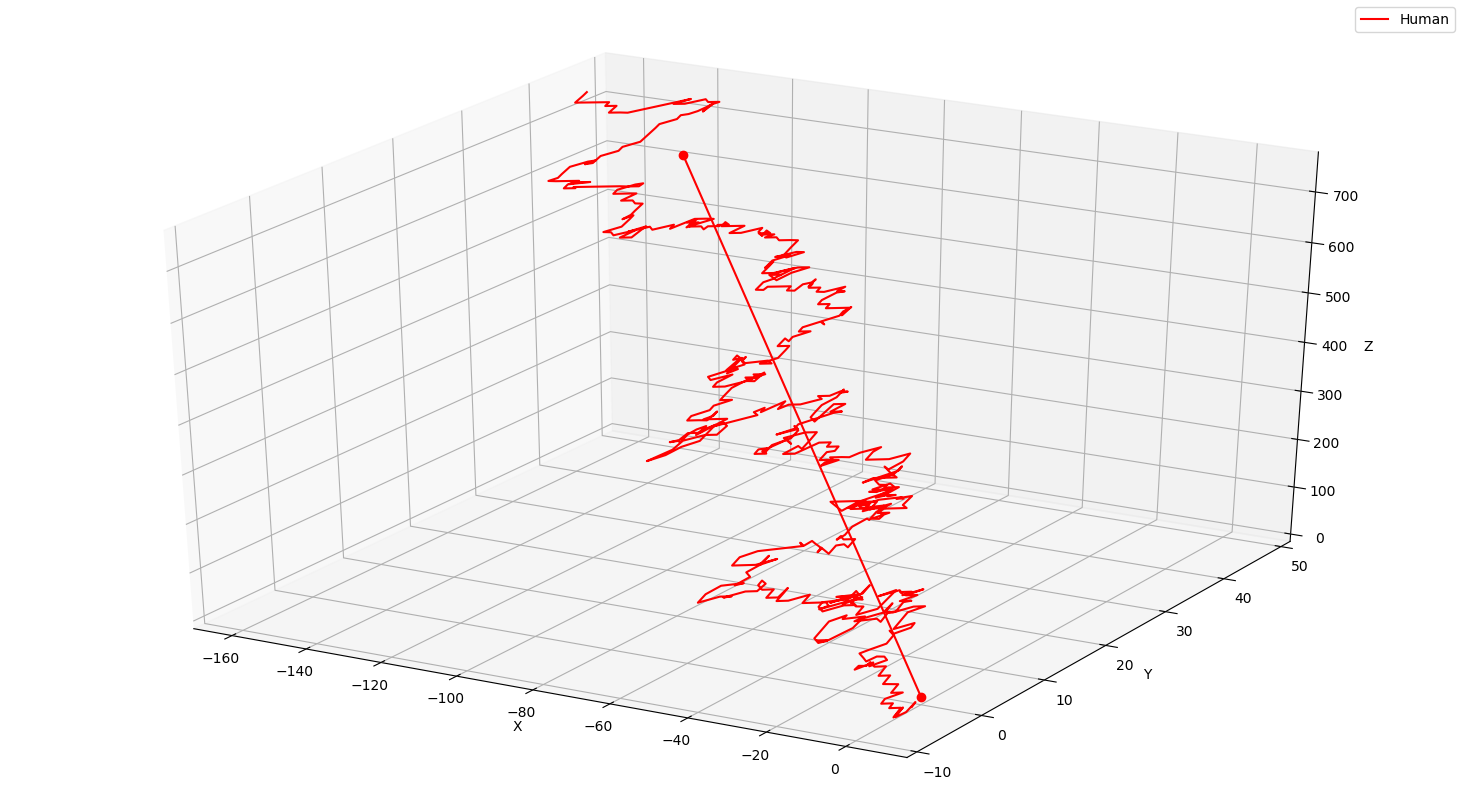
\includegraphics[width=70mm]{pic07.png}
\caption{ヒトのND5配列グラフと慣性主軸}
\end{figure}



\newpage
\section{配列間の距離}
配列間の類似性を定量的に評価するために距離を定義する。本研究では、それぞれの慣性主軸なす角を$θ$として$cosθ$を計算する。方向ベクトルを$\vec{a}$、$\vec{b}$とすると、$cosθ$は以下の式で求められる。

\begin{equation}
\cos = \frac{\vec{a}\cdot\vec{b}}{|\vec{a}||\vec{b}|}
\end{equation}

上記の式の値をアークコサインを用いて求めた$θ$の値を距離と定義した。


\chapter{結果}

\section{実験に用いたデータ}
本研究で使用した生物種は以前の研究[1]と同じ哺乳類の9種類で、以下の表の通りである。ミトゴンドリアDNAにコードされているNDAHデヒドロゲナーゼサブユニット5(以下ND5タンパク質)を使用した。

\begin{table}[H]
\centering
\caption{使用した生物種}
\scalebox{1}[1]{
\begin{tabular}{|l|c|c|} \hline
英名(和名)& accession no. & 配列長 \\ \hline
Human:ヒト & AP\_000649 & 603 \\[-2mm]
Gorilla:ゴリラ & NP\_008222 & 603 \\[-2mm]
Pygmy chimpanzee(P.chi.):ボノボ & NP\_008209 & 603 \\[-2mm]
Common chimpanzee(C.chi.):チンパンジー & NP\_008196 & 603 \\[-2mm]
Fin whale(F.wh.):ナガスクジラ & NP\_006899 & 606 \\[-2mm]
Blue whale(B.wh.):シロナガスクジラ & NP\_007066 & 606 \\[-2mm]
Rat:ドブネズミ & AP\_004902 & 610 \\[-2mm]
Mouse:ハツカネズミ  & NP\_904338 & 607 \\[-2mm]
Opposum(Oposs.):オポッサム & NP\_007105 & 602 \\ \hline
\end{tabular}}
\end{table}

\newpage
\section{グラフ表示}
図にそれぞれのアミノ酸の配置方法でグラフ化した3次元座標群を示す。

\begin{figure}[H]
\centering
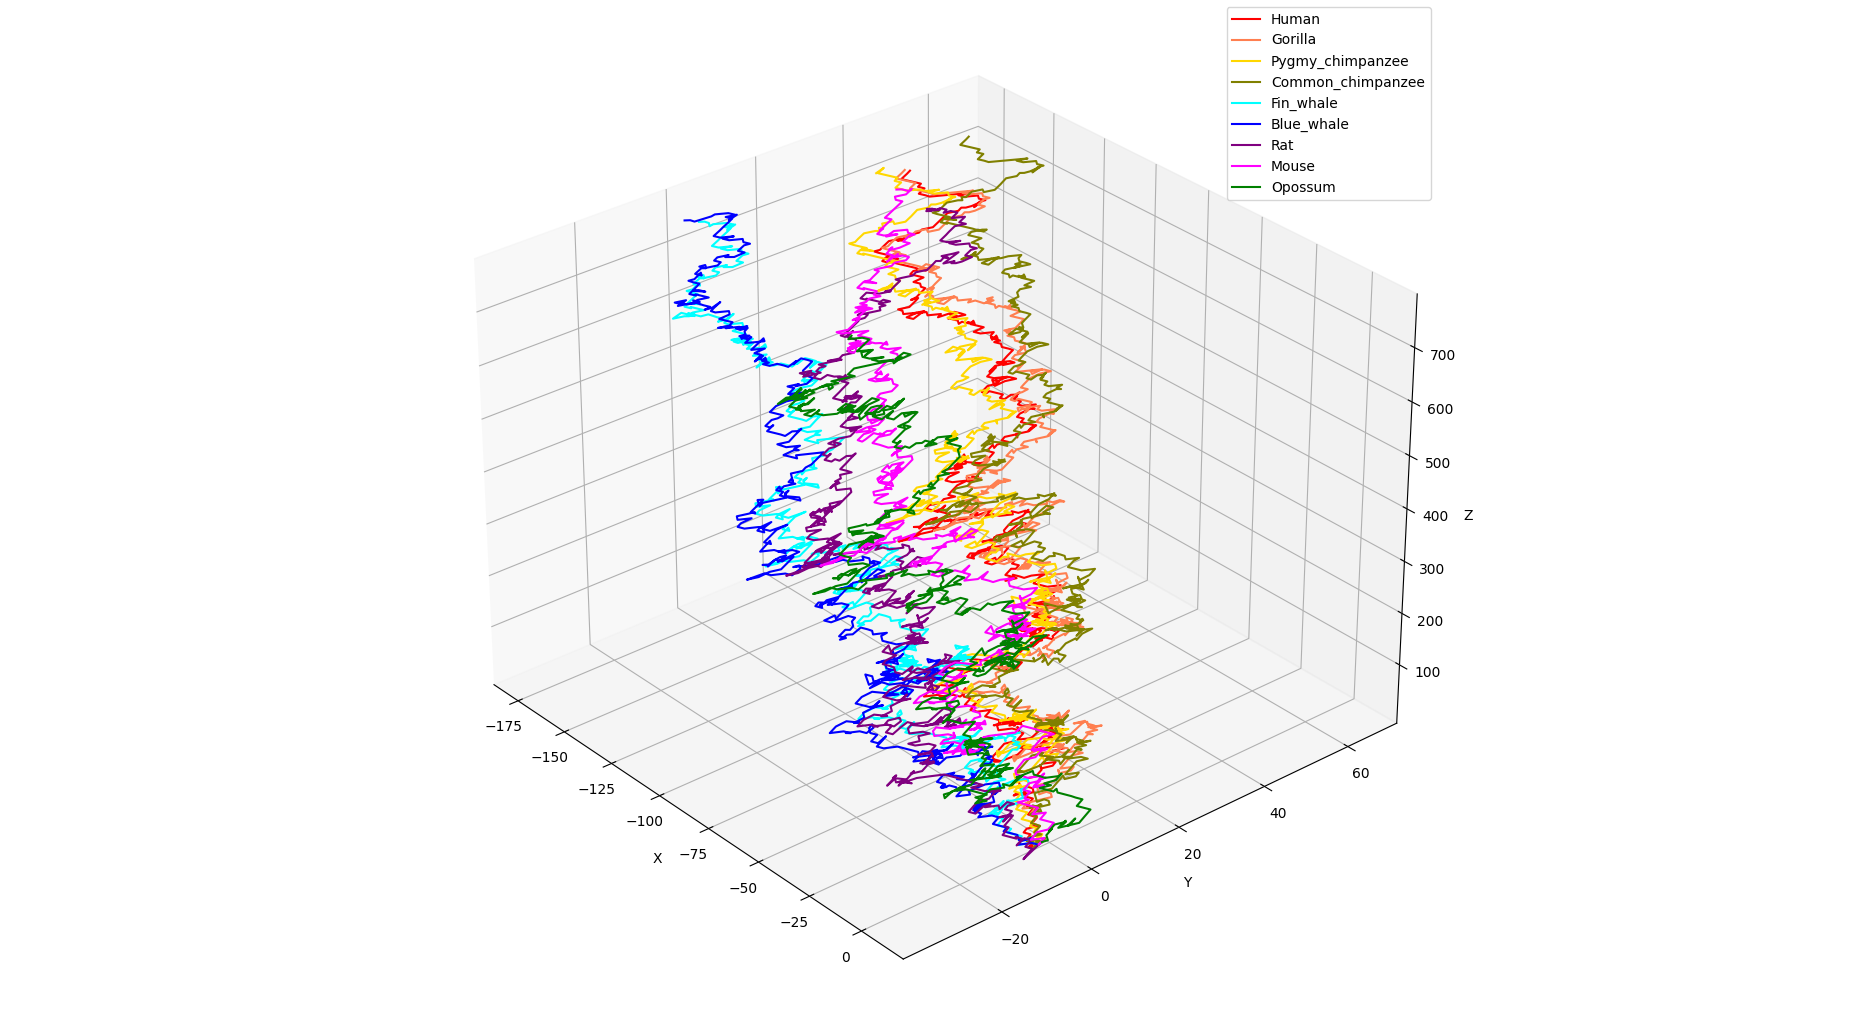
\includegraphics[width=120mm]{pic_graph_hydro1.png}
\caption{系統樹(アミノ酸を疎水性度の値が小さい順に、内側、外側に10種類ずつ二重円で配置)}
\end{figure}

\begin{figure}[H]
\centering
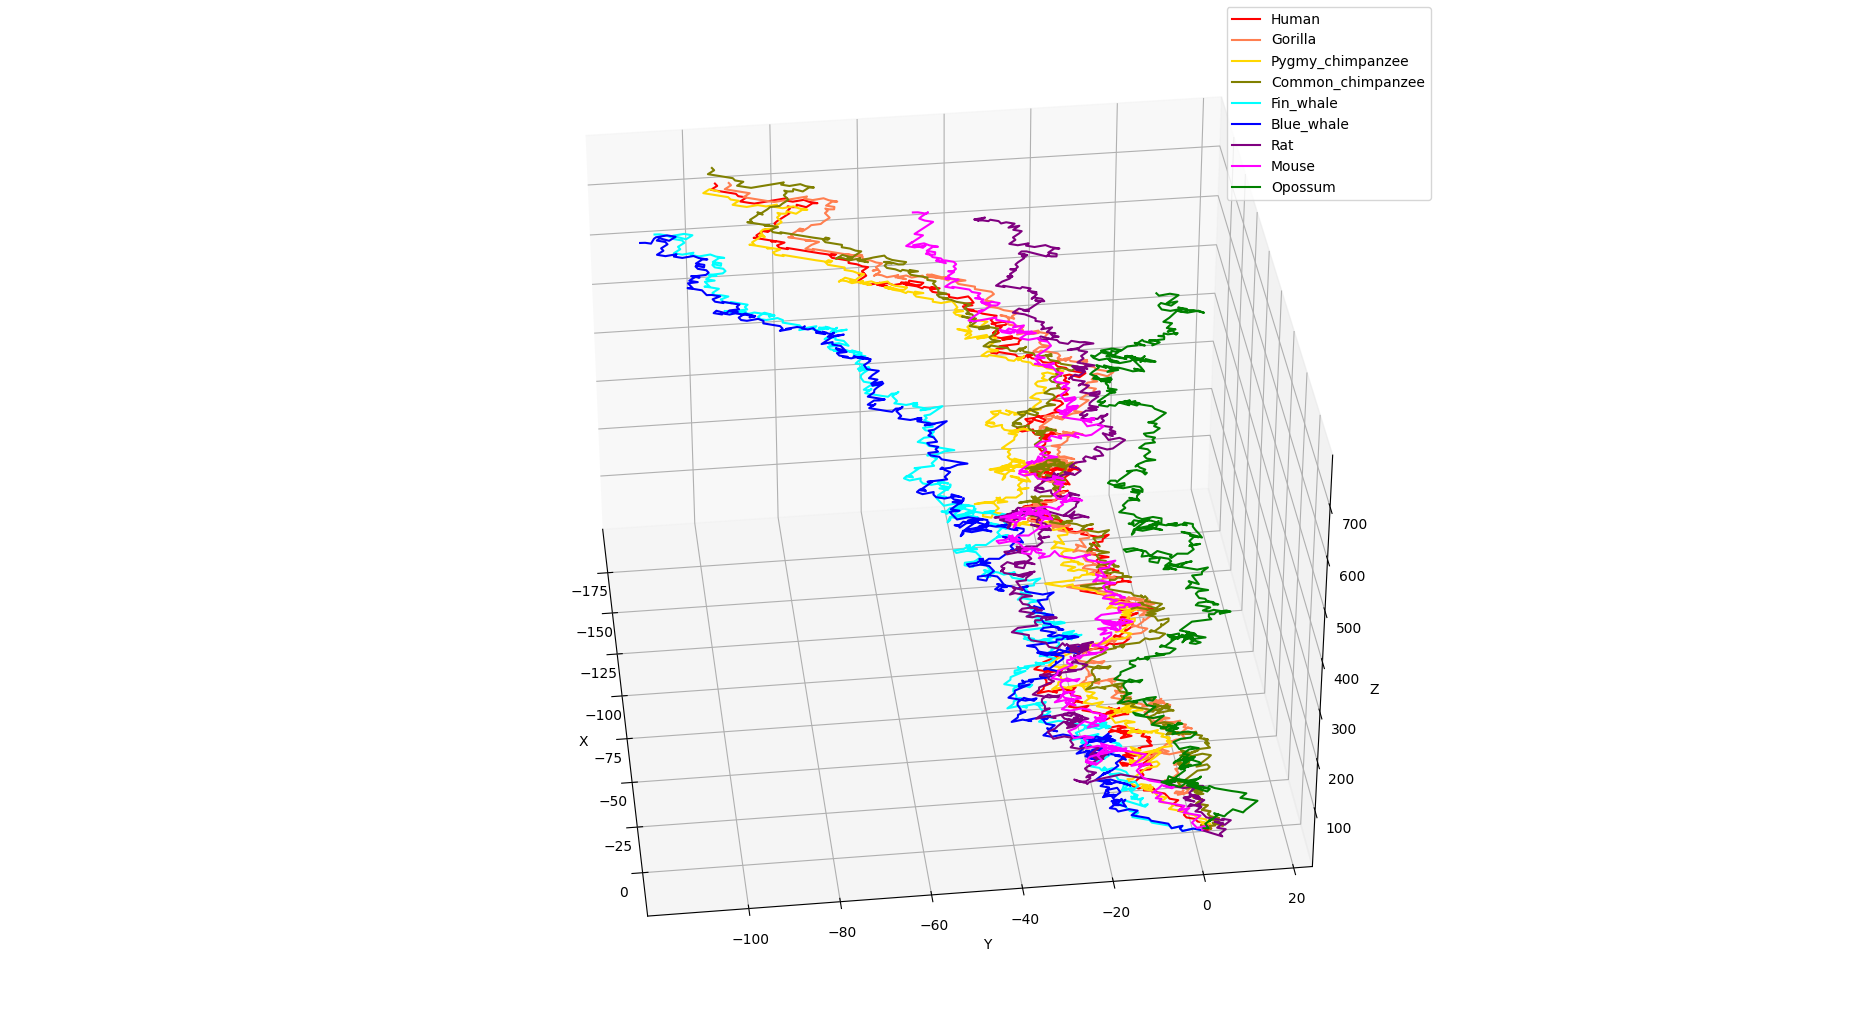
\includegraphics[width=120mm]{pic_graph_hydro2.png}
\caption{系統樹(アミノ酸を疎水性度の値が小さい順に、疎水性度の値がプラスとマイナスで分けて二重円に配値)}
\end{figure}

\begin{figure}[H]
\centering
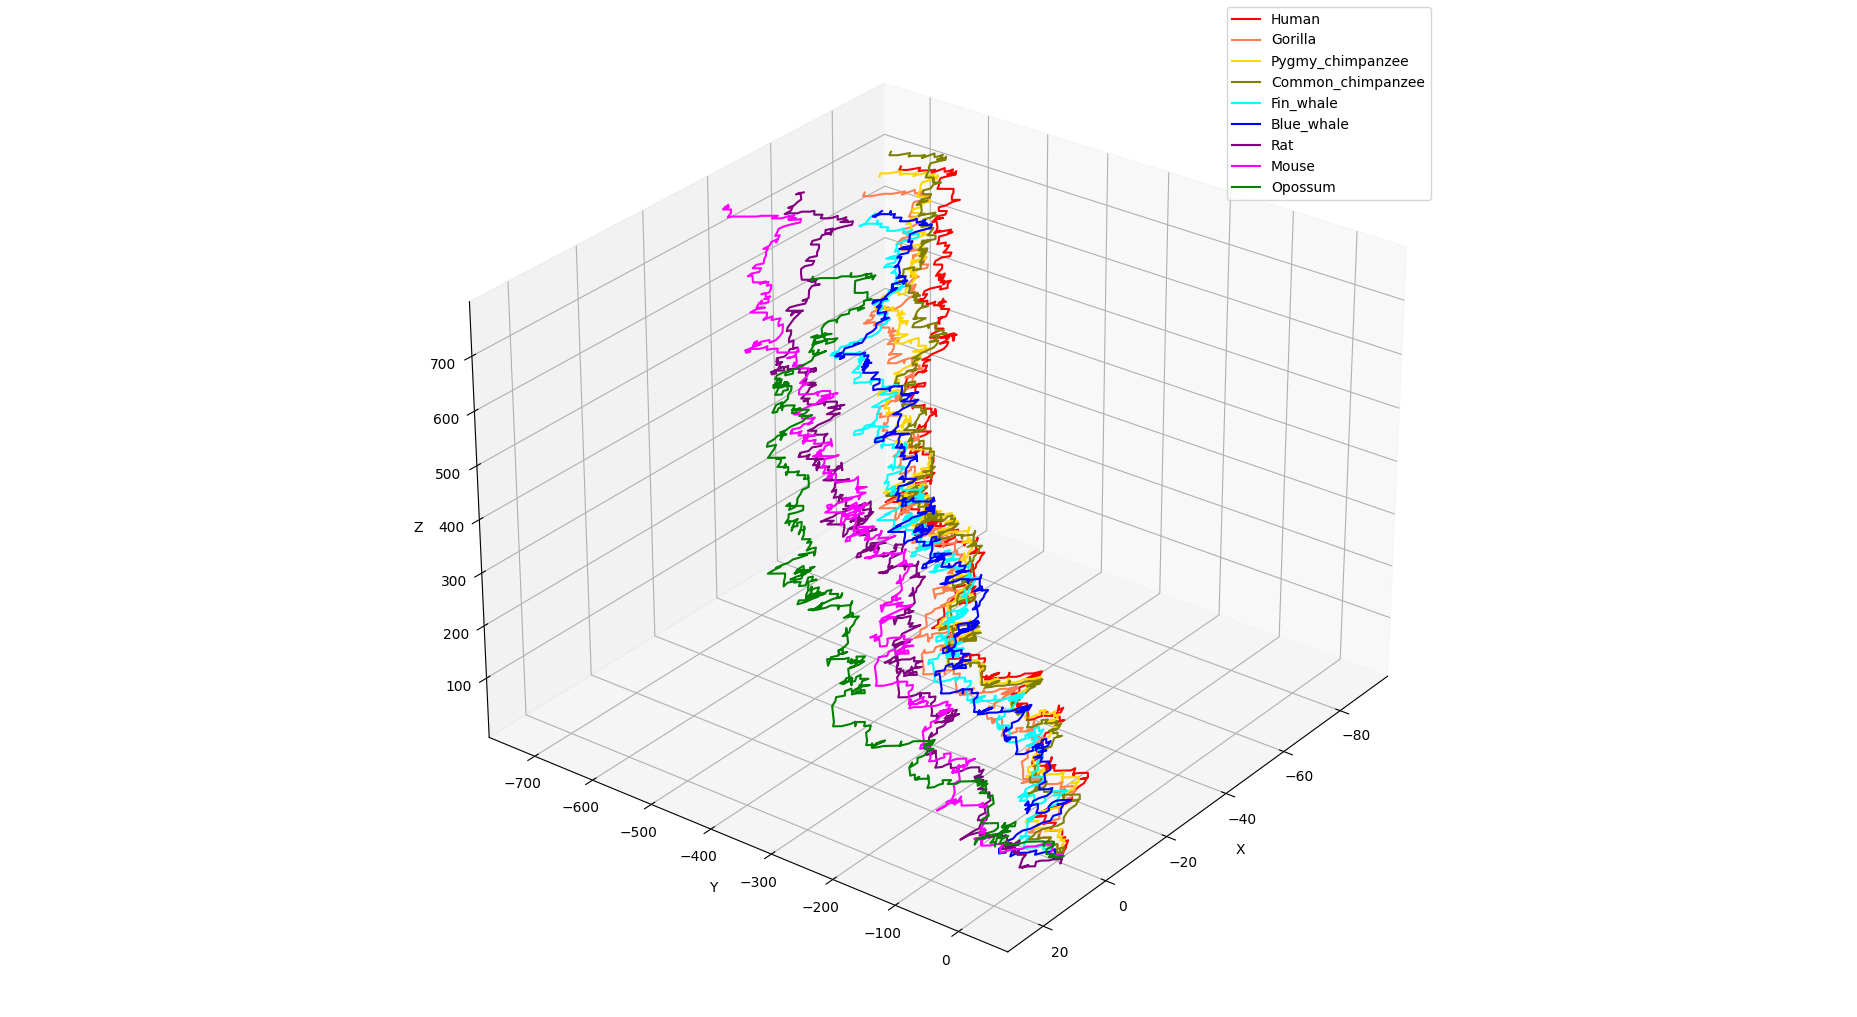
\includegraphics[width=120mm]{pic_graph_hydro3.png}
\caption{系統樹(アミノ酸を疎水性度の値が小さい順に、疎水性度の値がプラスとマイナスで分けて左右に配値)}
\end{figure}

\begin{figure}[H]
\centering
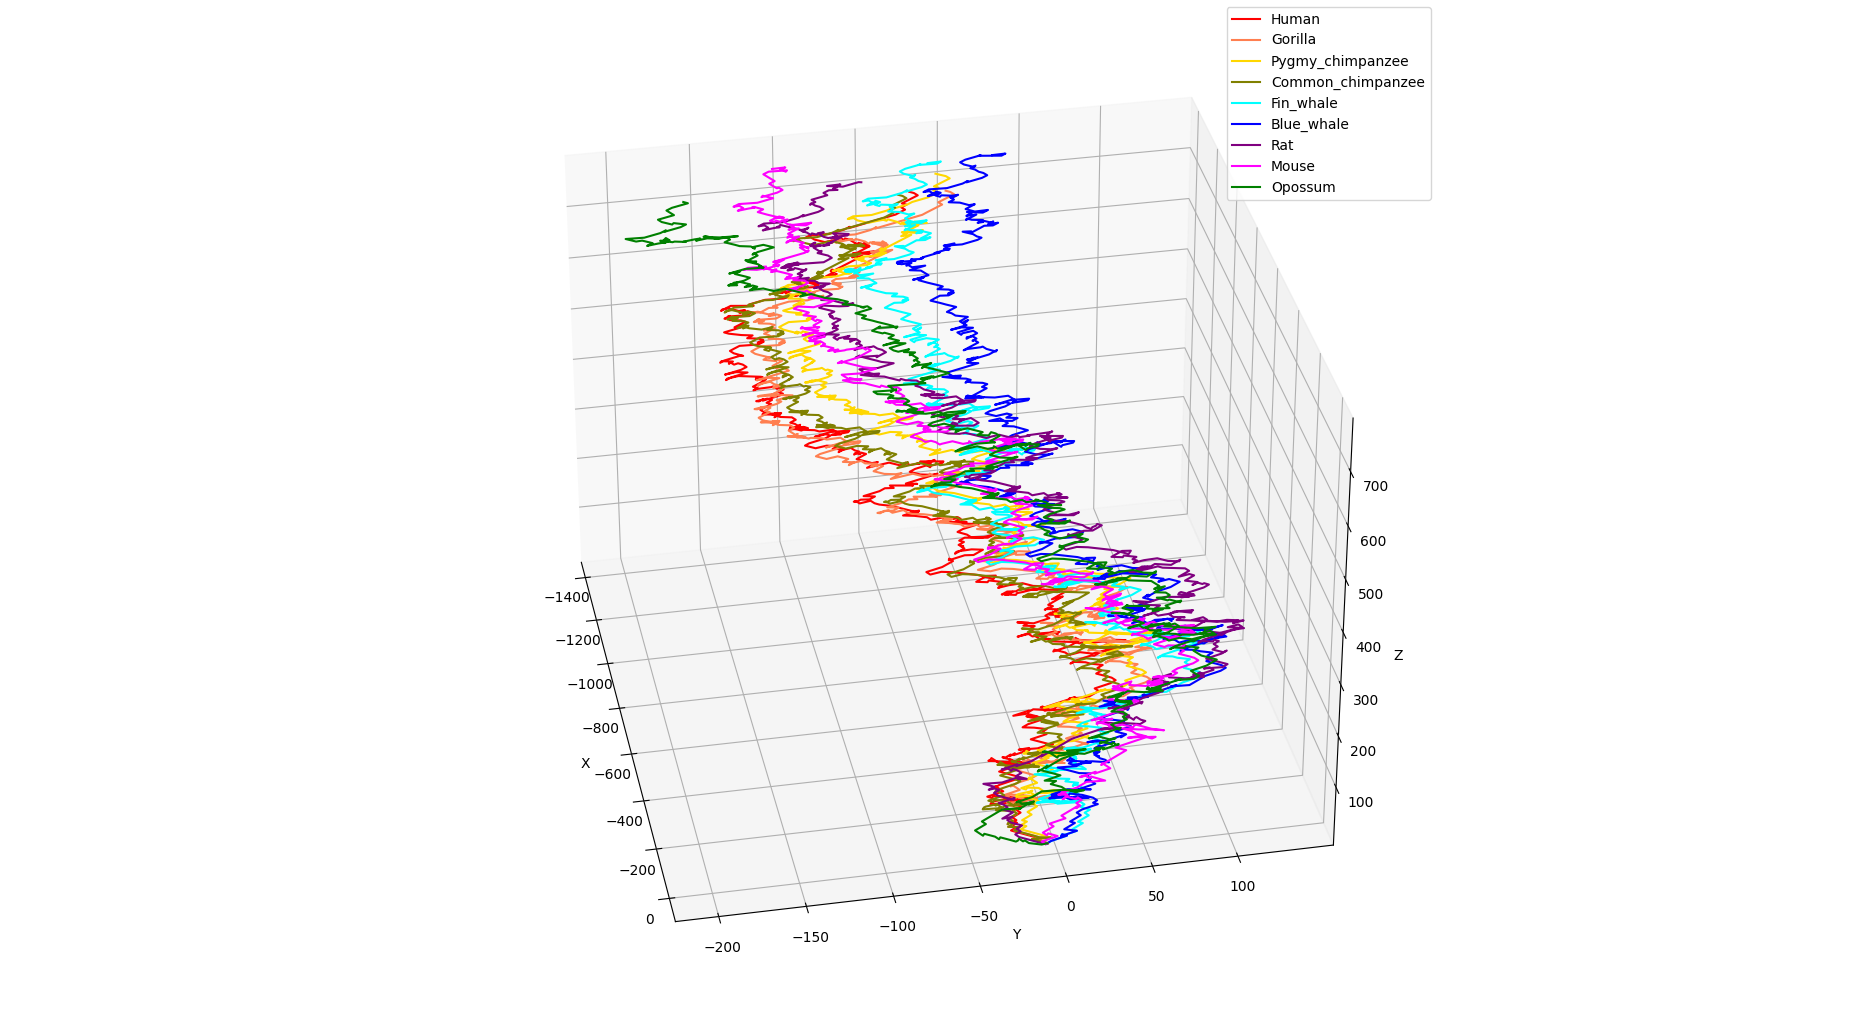
\includegraphics[width=120mm]{pic_graph_codon.png}
\caption{系統樹(コドン表)}
\end{figure}

\begin{figure}[H]
\centering
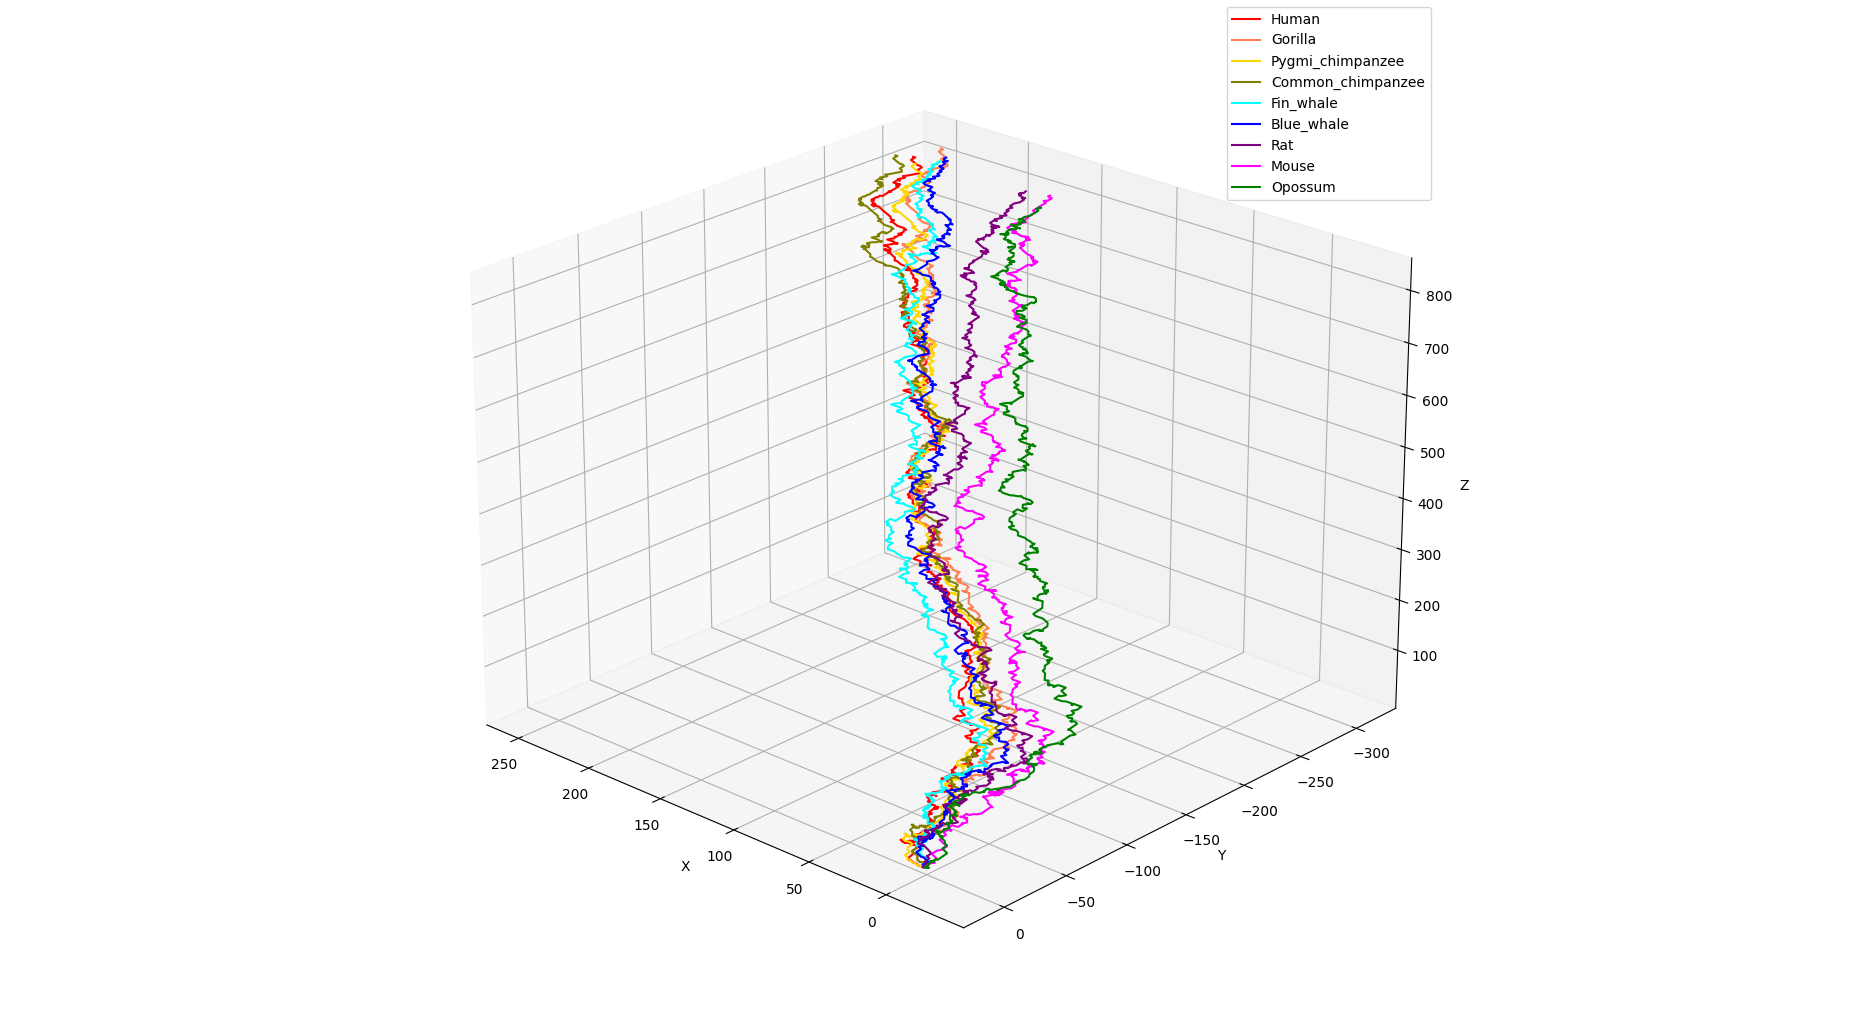
\includegraphics[width=120mm]{pic_graph_iso.png}
\caption{系統樹(等電点)}
\end{figure}

また、ヒトとゴリラのND5配列グラフと、ヒトとドブネズミの配列グラフを示す(配置:アミノ酸を疎水性度の値が小さい順に、内側、外側に10種類ずつ二重円)。近縁種同士のグラフの概形が似ていることが直観的にわかる。

\begin{figure}[H]
\centering
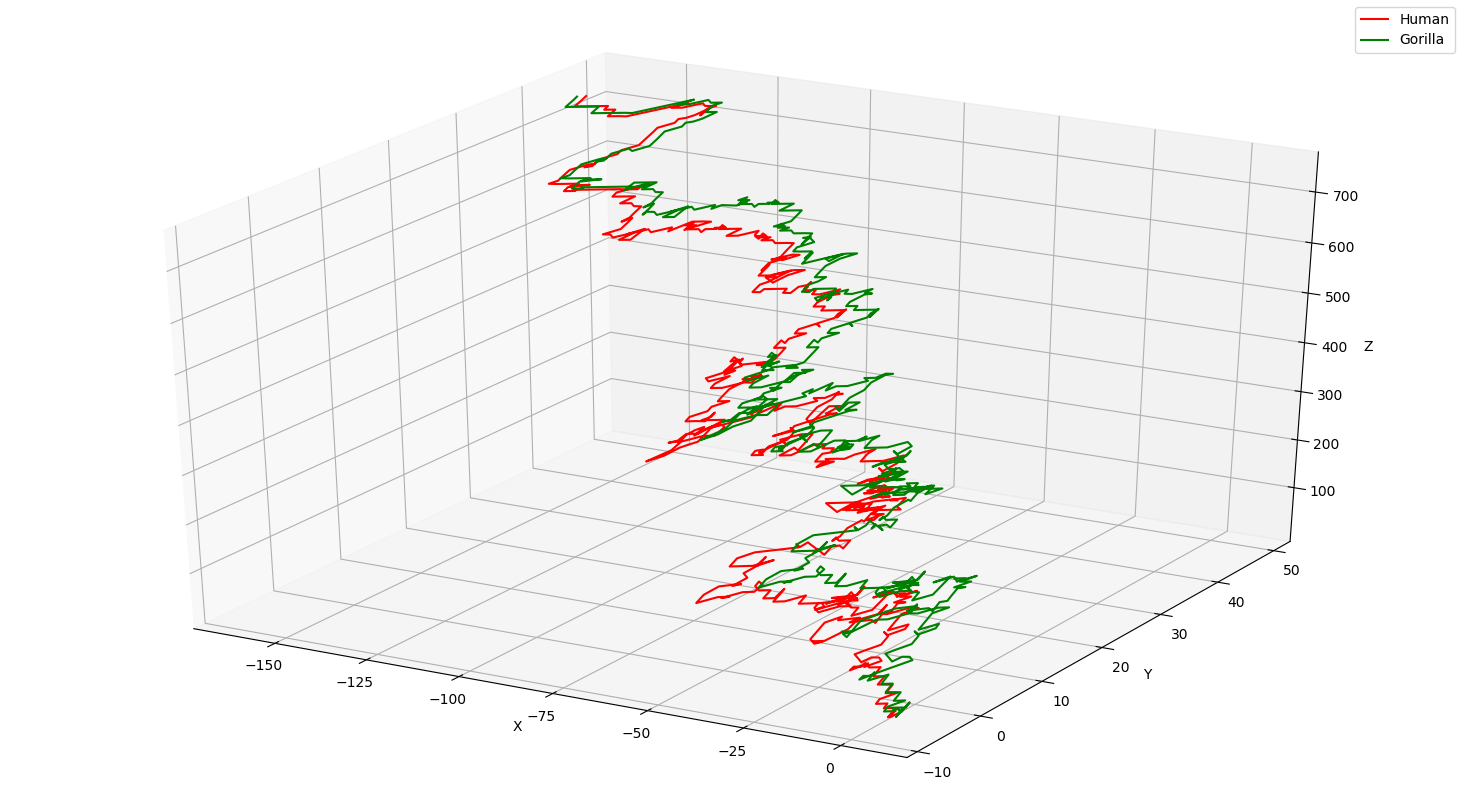
\includegraphics[width=120mm]{pic05.png}
\caption{ヒトとゴリラのND5配列グラフ}
\end{figure}

\begin{figure}[H]
\centering
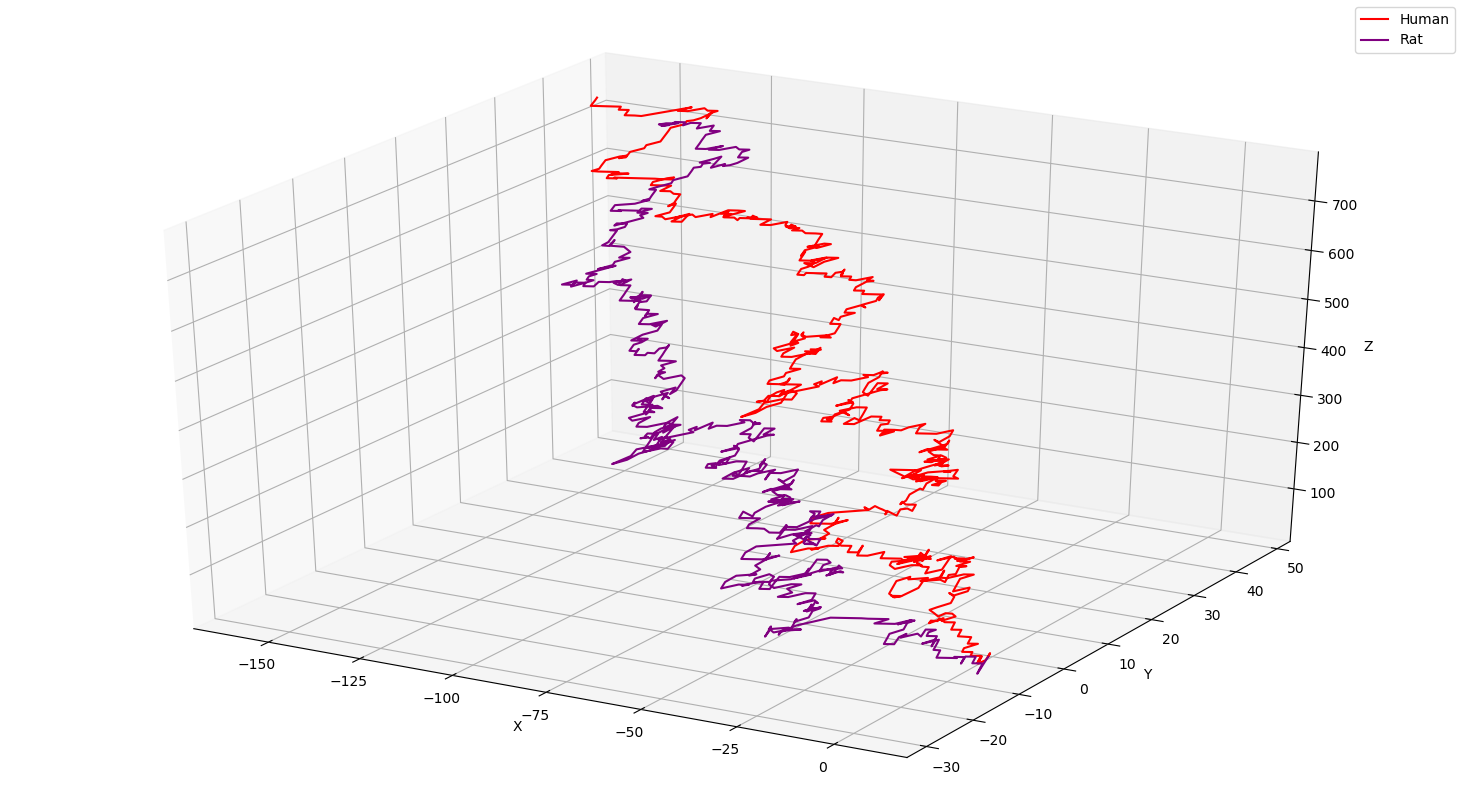
\includegraphics[width=120mm]{pic06.png}
\caption{ヒトとドブネズミの配列グラフ}
\end{figure}


\newpage
\section{距離行列}
表に距離行列を示す(配置:アミノ酸を疎水性度の値が小さい順に、内側、外側に10種類ずつ二重円)。近縁種同士は距離が近く、遠縁種になるほど距離が距離が遠くなる。

\begin{table}[H]
\centering
\caption{距離行列}
\scalebox{0.7}[0.7]{
\begin{tabular}{|c|c|c|c|c|c|c|c|c|c|} \hline
 & Human & Gorilla & P.chi. & C.chi. & F.wh. & B.wh. & Rat & Mouse & Oposs. \\ \hline
Human & 0.000000  & &  & & & & & &  \\ 
Gorilla & 0.005051  & 0.000000  & & & & & & &  \\ 
P.chi. & 0.015240  & 0.010324  & 0.000000  & &  & & & &  \\ 
C.chi. & 0.037277  & 0.034013  & 0.031824  & 0.000000  & & & & &  \\
F.wh. & 0.060044  & 0.056226  & 0.047202  & 0.068429  & 0.000000  & & & &  \\ 
B.wh. & 0.056720  & 0.052415  & 0.042636  & 0.060392  & 0.009848  & 0.000000  & & &  \\ 
Rat & 0.034017  & 0.038222  & 0.045817  & 0.070978  & 0.076177  & 0.077046  & 0.000000  & &  \\ 
Mouse & 0.033555  & 0.035730  & 0.039368  & 0.069580  & 0.059244  & 0.061471  & 0.018854  & 0.000000  &  \\ 
Oposs. & 0.083178  & 0.086221  & 0.090629  & 0.120227  & 0.099408  & 0.105021  & 0.052022  & 0.051262  & 0.000000  \\ \hline
\end{tabular}}
\end{table}


\newpage
\section{系統樹}
PhylipでUPGMA法を用いて系統樹を作成した。


\begin{figure}[H]
\centering
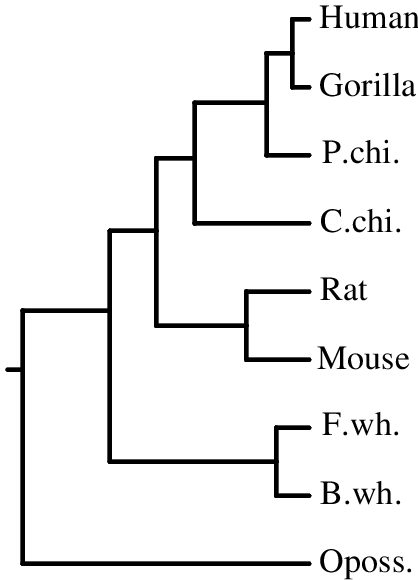
\includegraphics[width=50mm]{picx1.png}
\caption{系統樹(アミノ酸を疎水性度の値が小さい順に、内側、外側に10種類ずつ二重円で配置)}
\end{figure}

\begin{figure}[H]
\centering
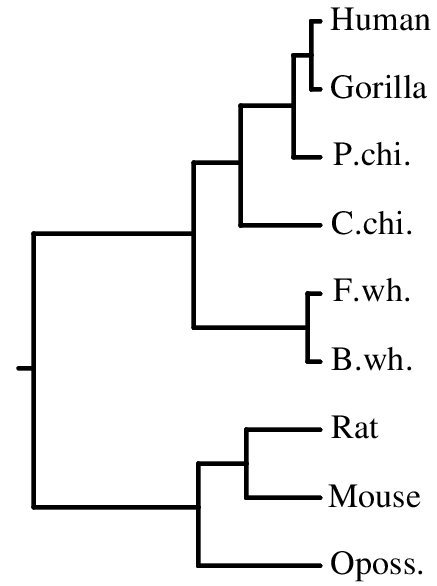
\includegraphics[width=50mm]{picx2.png}
\caption{系統樹(アミノ酸を疎水性度の値が小さい順に、疎水性度の値がプラスとマイナスで分けて二重円に配値)}
\end{figure}

\begin{figure}[H]
\centering
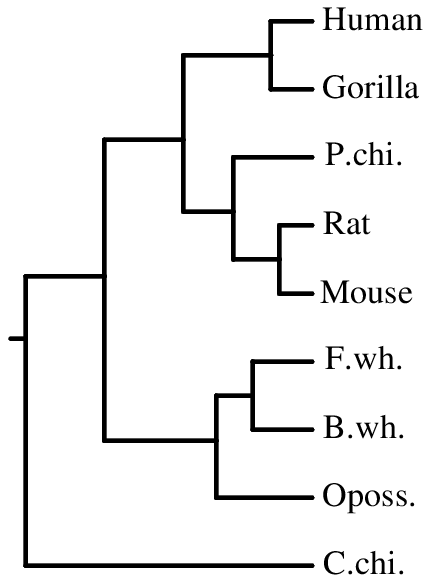
\includegraphics[width=50mm]{picx3.png}
\caption{系統樹(アミノ酸を疎水性度の値が小さい順に、疎水性度の値がプラスとマイナスで分けて左右に配値)}
\end{figure}

\begin{figure}[H]
\centering
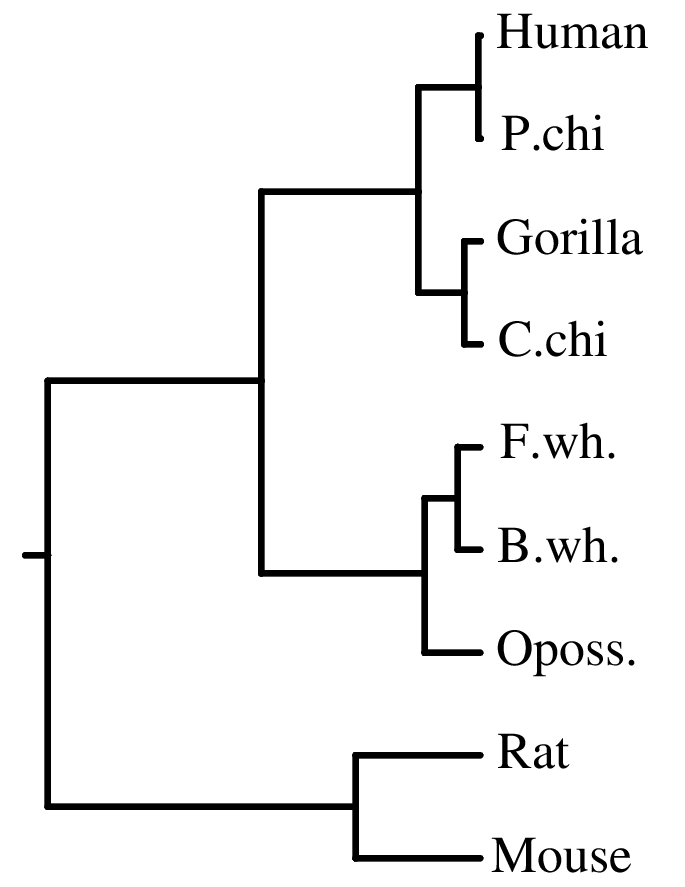
\includegraphics[width=50mm]{picx4.png}
\caption{系統樹(コドン表)}
\end{figure}

\begin{figure}[H]
\centering
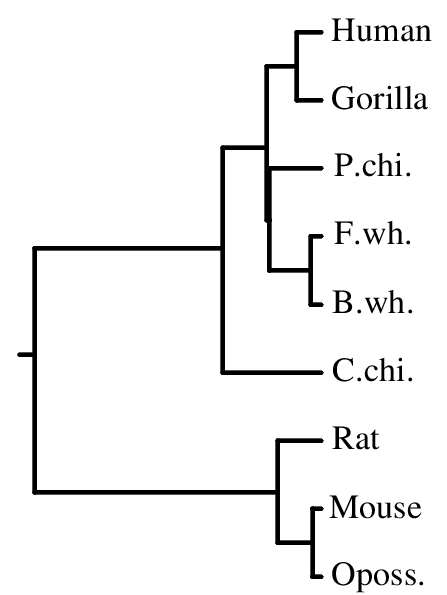
\includegraphics[width=50mm]{picx6.png}
\caption{系統樹(等電点)}
\end{figure}

\begin{figure}[H]
\centering
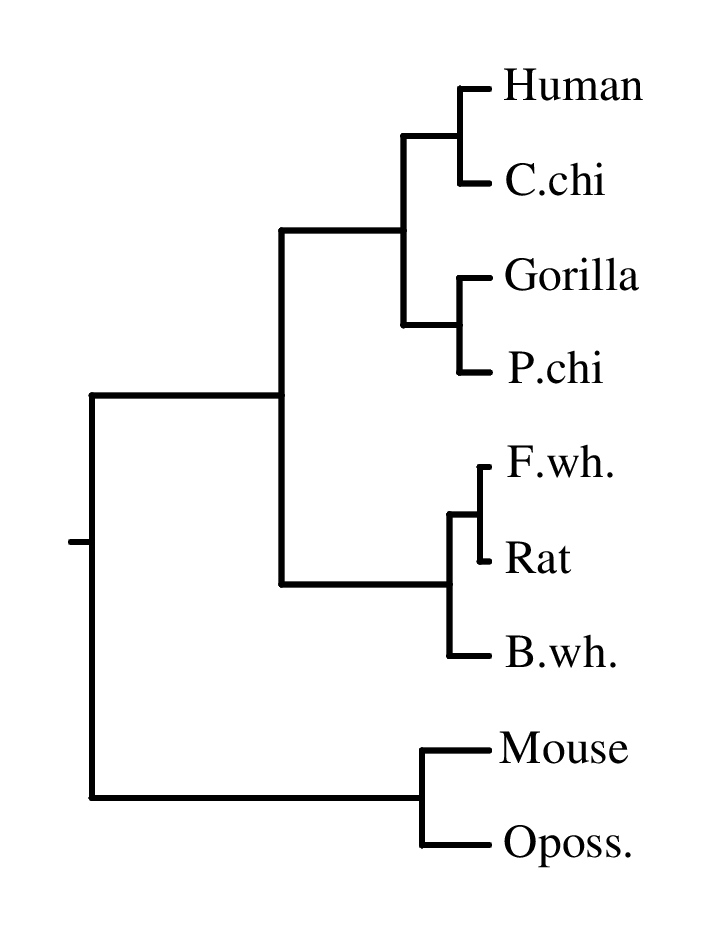
\includegraphics[width=50mm]{picx5.png}
\caption{系統樹(参考文献[1])}
\end{figure}

\chapter{まとめと今後の課題}
本研究では、タンパク質のアミノ酸配列を3次元座標化し、その慣性主軸をのなす角から距離を計算した。近縁種同士はグラフの概形が似ており、直観的に近縁種なのか遠縁種なのか判断し、3次元グラフの慣性主軸を特徴量とすることで配列間を定量的に評価できた。\\
 アミノ酸に割り当てるベクトル配置を複数検討することにより、より正確な系統樹を作成した。アミノ酸を疎水性度の値が小さい順に、内側、外側に10種類ずつ二重円で配置したときは、系統樹に矛盾がなく、現段階で最も正確な系統樹となった。アミノ酸を疎水性度の値が小さい順に、値がプラスとマイナスで分けて二重円に配値したときは、外縁であるオポッサムが齧歯目のツリーに入ってしまった。アミノ酸を疎水性度の値が小さい順に、値がプラスとマイナスで分けて左右に配値したときは、齧歯目がボノボ、オポッサムがクジラと近縁になっており、チンパンジーが外縁となった。コドン表を元にした配置したときは、オポッサムとクジラが近縁となった。等電点を元に配置したときは、チンパンジーとクジラ、齧歯目がオポッサムと近縁となった。\\
 今後の課題として、生物種を増やしたときに正確な系統樹ができないという問題が挙げられる。本研究では9種類の生物種を取り扱ったが、19種類に増やしたときに完全な分類ができなかった。そのため、生物種を増やしたときにも対応できるよう、より正確な指標・配置を見つける必要がある。例えば、疎水性度と相関のない指標を探すことなどが考えられる。他には、z座標も配置の変更に使う、ND5タンパク質ではないタンパク質を用いるなどが考えられる。

\begin{thebibliography}{9}
\bibitem{agata} Agata,C ,Dorota,B ,Piotr,W and Tim,C "20D-dynamic representation of protein sequences" Ge-nomics Volume 107, Issue 1, January 2016, Pages 16-23
\bibitem{mizuta} Mizuta,S "Graphical Representation of Biological Sequences" (2018)
\end{thebibliography}



\end{document}








